\chapter{Vector Analysis}
\section{Vector Algebra}

\section{Differential Calculus}
\subsection{"Ordinary Derivatives"s}
\subsection{Gradient}
\subsection{The Del Operator}
\subsection{The Divergence}
\subsection{The Curl}
\subsection{Product Rules}
\subsection{Second Derivatives}
\section{Integral Calculus}

\section{Curvilinear Coordinates}
\subsection{Spherical Coordinates}
\subsection{Cynlindrical Coordinates}

\section{The Dirac Delta Function}
\subsection{The Divergence of $\frac{\hat{r}}{r^{2}}$}
\begin{equation}
\nabla . \frac{\hat{r}}{r^{2}} = 0
\end{equation}
\subsection{The One-Dimensional Dirac Delta Function}
The Dirac Delta is a functional \footnote{An object that is a map between functions} which we define as,
\begin{equation}
\delta(x-a)= 
\begin{cases}
0, & \text{if } x \neq a\\
\infty,              & \text{if } x = a
\end{cases}
\label{del1}
\end{equation}
\begin{equation}
\int_{- \infty}^{+ \infty} \delta(x-a) dx = 1
\label{del2}
\end{equation}
$\forall \  a \in \mathbb{R}$
We can visualize it as a sharp peak at $a$,
\begin{figure}
\centering
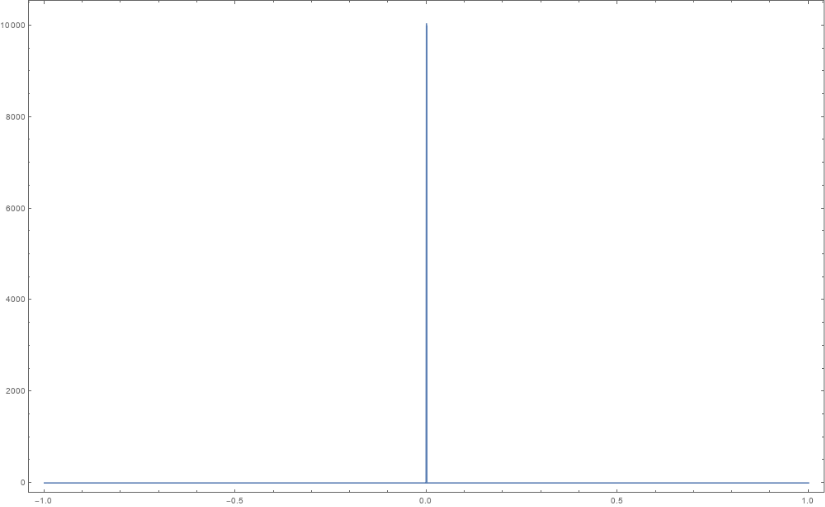
\includegraphics[scale=0.5]{delta-distribution.png}
\caption{A Plot of $\delta(x)$}
\end{figure}
We can interpret \ref{del2} as saying "the area of the delta distribution is always 1".
\begin{equation}
f(x)\delta(x - a ) = f(a)
\end{equation}
We can combine these to get,
\begin{equation}
\int_{- \infty}^{+ \infty} \delta(x-a) f(x) dx = f(a)
\end{equation}
\subsubsection{A few interesting properties}
\begin{equation}
\delta(kx) = \frac{1}{|k|}\delta(x)
\end{equation}
\begin{equation}
\frac{d}{dx}(\delta(x)) = -\delta(x)
\end{equation}
where k is a constant
\begin{equation}
\frac{d \theta}{dx} = \delta(x)
\end{equation}
Where $\theta$ is the step function defined as,
\begin{equation}
\theta(x)= 
\begin{cases}
1, & \text{if } x > 0\\
o,              & \text{if } x \leq 0
\end{cases}
\end{equation}

\subsection{The Three-Dimensional Dirac Delta Function}
We generalize () to three dimensions,
\begin{equation}
\delta^{3}(\vec{r} - \vec{a}) = \delta(x-a_{x})\delta(y-a_{y})\delta(z-a_{z})
\end{equation}
\begin{equation}
\int_{- \infty}^{+ \infty} \delta^{3}(\vec{r} - \vec{a}) dV = 1
\end{equation}
We can also define the three-dimensional delta function as
\begin{equation}
\mathfrak{r}
\end{equation}
$$\mathfrak{r} = $$
\section{The Theory of Vector Fields}
\subsection{The Helmoltz Theorem}
This does cause an issue with "Ontology" \footnote{What's real and what isn't?}
\subsection{Potentials}